%%%%%%%%%%%%%%%%%%%%%%%%%%%%%%%%%%%%%%%%%
% University Assignment Title Page 
% LaTeX Template
% Version 1.0 (27/12/12)
%
% This template has been downloaded from:
% http://www.LaTeXTemplates.com
%
% Original author:
% WikiBooks (http://en.wikibooks.org/wiki/LaTeX/Title_Creation)
%
% License:
% CC BY-NC-SA 3.0 (http://creativecommons.org/licenses/by-nc-sa/3.0/)
% 
% Instructions for using this template:
% This title page is capable of being compiled as is. This is not useful for 
% including it in another document. To do this, you have two options: 
%
% 1) Copy/paste everything between \begin{document} and \end{document} 
% starting at \begin{titlepage} and paste this into another LaTeX file where you 
% want your title page.
% OR
% 2) Remove everything outside the \begin{titlepage} and \end{titlepage} and 
% move this file to the same directory as the LaTeX file you wish to add it to. 
% Then add \input{./title_page_1.tex} to your LaTeX file where you want your
% title page.
%
%%%%%%%%%%%%%%%%%%%%%%%%%%%%%%%%%%%%%%%%%

%----------------------------------------------------------------------------------------
%	PACKAGES AND OTHER DOCUMENT CONFIGURATIONS
%----------------------------------------------------------------------------------------

\documentclass[12pt]{article}

\usepackage{graphicx}

\begin{document}

\begin{titlepage}

\newcommand{\HRule}{\rule{\linewidth}{0.5mm}} % Defines a new command for the horizontal lines, change thickness here

\center % Center everything on the page
 
%----------------------------------------------------------------------------------------
%	HEADING SECTIONS
%----------------------------------------------------------------------------------------

\textsc{\LARGE Barcelona Graduate School}\\[0.2cm] % Name of your university/college
\textsc{\LARGE of Economics}\\[1.5cm] % Name of your university/college
\textsc{\Large Masters Project}\\[0.5cm] % Major heading such as course name
\textsc{\large }\\[0.5cm] % Minor heading such as course title

%----------------------------------------------------------------------------------------
%	TITLE SECTION
%----------------------------------------------------------------------------------------

\HRule \\[0.4cm]
{ \huge \bfseries Combinatorial Bandit}\\[0.4cm] % Title of your document
{ \huge \bfseries Algorithms in Practice}\\[0.4cm]
\HRule \\[1.5cm]
 
%----------------------------------------------------------------------------------------
%	AUTHOR SECTION
%----------------------------------------------------------------------------------------

%\begin{minipage}{0.4\textwidth}
%\begin{flushleft} \large
%\emph{Authors:}\\
%Angus \textsc{McKay} % Your name
%Akhil \textsc{Lohia} % Your name
%\end{flushleft}
%\end{minipage}
%~
%\begin{minipage}{0.4\textwidth}
%\begin{flushright} \large
%\emph{Supervisor:} \\
%Dr. James \textsc{Smith} % Supervisor's Name
%\end{flushright}
%\end{minipage}\\[4cm]

% If you don't want a supervisor, uncomment the two lines below and remove the section above
\Large \emph{Authors:}\\
Angus \textsc{McKay}\\ % Your name
Akhil \textsc{Lohia}\\[3cm] % Akhil's name

%----------------------------------------------------------------------------------------
%	DATE SECTION
%----------------------------------------------------------------------------------------

{\large \today}\\[3cm] % Date, change the \today to a set date if you want to be precise

%----------------------------------------------------------------------------------------
%	LOGO SECTION
%----------------------------------------------------------------------------------------

%\includegraphics{Logo}\\[1cm] % Include a department/university logo - this will require the graphicx package
 
%----------------------------------------------------------------------------------------

\vfill % Fill the rest of the page with whitespace

\end{titlepage}

%----------------------------------------------------------------------------------------
%	ABSTRACT PAGE
%----------------------------------------------------------------------------------------

\section{Abstract}
%\addchaptertocentry{\abstractname} % Add the abstract to the table of contents


There has recently been a lot of interest in online learning algorithms where limited feedback is received at each stage of the process, known as bandit problems. Such algorithms generally choose a subset of available options to 'play' at each round. For the options chosen, some stochastic reward (or cost) is returned. In a semi-bandit situation, the reward is observed for each option which is played. In a full-bandit scenario, only the total reward is observed. A lot of practical problems also contain a combinatorial element to them, whereby a combinatorial problem needs to be solved using the feedback observed.\\

Recent literature has proposed many different algorithms and approaches for these bandit problems. The literature is also full of mathematical proofs for bounds on regret risk (i.e. the difference between a chosen solution and the optimal solution). However, there is relatively little information on how these algorithms perform in practice. This paper intends to explore the performance of some of the proposed approaches in a more practical setting. 

\pagebreak

\vfill % Fill the rest of the page with whitespace

%----------------------------------------------------------------------------------------
%	ACKNOWLEDGEMENTS
%----------------------------------------------------------------------------------------

\section{Acknowledgements}
%\addchaptertocentry{\acknowledgementname} % Add the acknowledgements to the table of contents
The acknowledgments and the people to thank go here

\pagebreak

%----------------------------------------------------------------------------------------
%	LIST OF CONTENTS/FIGURES/TABLES PAGES
%----------------------------------------------------------------------------------------

\tableofcontents % Prints the main table of contents

\pagebreak

%----------------------------------------------------------------------------------------
%	INTRO
%----------------------------------------------------------------------------------------

\section{Introduction}

Online learning

Deterministic/stochastic/adversary

Combinatorial element and optimization oracle

Exploration vs exploitation

Examples


\pagebreak

%----------------------------------------------------------------------------------------
%	ALGORITHMS
%----------------------------------------------------------------------------------------

\section{Algorithms}

\subsection{CombUCB1}

One of the most well-known algorithms for multi-armed bandit problems is UCB1. This has been adapted to the combinatorial setting by Kveton et al [1], who developed combUCB1. After each iteration the algorithm calculates a confidence bound around the empirical mean reward/cost of each element. These confidence bounds are then used in the combinatorial optimization problem, the solution which is the chosen play for the next round. The more observations that are available of an element, the tighter the confidence bound around the expeceted value. Loosely speaking, relatively unobserved items will have larger confidence bounds so they will be explored until ther is more confidence in their expected value.\\

The confidence intervals are calculated as:

$$\hat{w}_t(e)\pm c_{t-1,e}$$ where $\hat{w}_{t-1}(e)$ is the average of the observations of option $e$ up to time $t-1$. $c_{t-1,e}$ is calculated as:

$$c_{t-1,e}=\sqrt{\frac{1.5\textrm{log}(t-1)}{n_{t-1}(e)}}$$ where $n_{t-1}(e)$ is the number of times that option $e$ has been observed up to time $t-1$.\\

The algorithm is set out formally below.

\noindent \hrulefill

\noindent \textbf{CombUCB1} algorithm for combinatorial semi-bandit problems

\noindent \hrulefill

\noindent \textit{Initialization}:

$\mathbf{\hat{w}}_0 \leftarrow$ make one observation of each edge

$n_0(e) \leftarrow 1$ $\forall$ $e \in E$\\

\noindent \textit{For all t in 1,...,T}:

Compute confidence intervals for each edge:

\indent \indent $U_t(e) \leftarrow \hat{w}_t(e)\pm c_{t-1,e}$ $\forall$ $e \in E$\\

Solve the optimization problem:

\indent \indent $A_t \leftarrow \textrm{arg max}_{A\in \Theta}f(A,U_t)$\\

Observe the weights of chosen items:

\indent \indent $w_t(e) \sim P_e$ $\forall$ $e \in A_t$

\indent \indent $w_t(e)=0$ otherwise\\

Update counts and expected values for each edge:

\indent \indent $n_t(e) \leftarrow n_{t-1}(e) + 1$ $\forall$ $e \in A_t$

\indent \indent $\hat{w}_t(e) \leftarrow \frac{n_{t-1}(e)\hat{w}_{t-1}(e)+w_t(e)}{n_t(e)}$ $\forall$ $e \in E$

\noindent \hrulefill\\

This assumes that one is able to initialize by choosing to observe each edge at least once before starting the algorithm. In practice if this is not feasible then the algorithm will produce a similar output if the initial weight for each edge is assumed to be the maximum (if a maximization problem) or minimum (if a minimization problem) values of the system (but these initial values are then disregarded in the algorithm once an observation has been made).\\

Note that the algorithm is computationally efficient, provide that the optimization problem step is. All other operations are polynomial in L and K.\\

<><><>TO DO - MAKE SURE EVERYTHING IS DEFINED PROPERLY EARLIER ON<><><>


FPL-TRiX

Others

Mathematical results (bounds etc)	


\pagebreak

%----------------------------------------------------------------------------------------
%	BASIC TESTING
%----------------------------------------------------------------------------------------

\section{Basic Testing}

\subsection{Basic stochastic setting}

For some initial insight into how the algorithms work in practice we can set up a basic simulation with a trivial "combinatorial" element. In this scenario we will have a vector of length L, and at each round K elements of this vector will be chosen. The weights of each chosen element will then be drawn from a Bernoulli distribution which will have a different mean for each element. A real-life application of such a system could be arranging adverts on a website where only K out of L adverts can be shown at any one time, and the goal is to maximise the number of times a user clicks on a link in an advert.\\

We start by setting L = 20, K = 5 and set the means as incrementally increasing values from 1/20 for the first element to 1 for the last element (so they are 1/20, 2/20, ..., 18/20, 19/20, 1). The game is to maximise the weights observed at each round. Clearly the optimal elements to play at each round are the last 5 elements as they have the highest probability of being drawn as 1. Let us observe how the algorithms explore the different options at different stages.\\


\noindent \textbf{UCB1}\\

\begin{figure}%                 use [hb] only if necceccary!
  \centering
  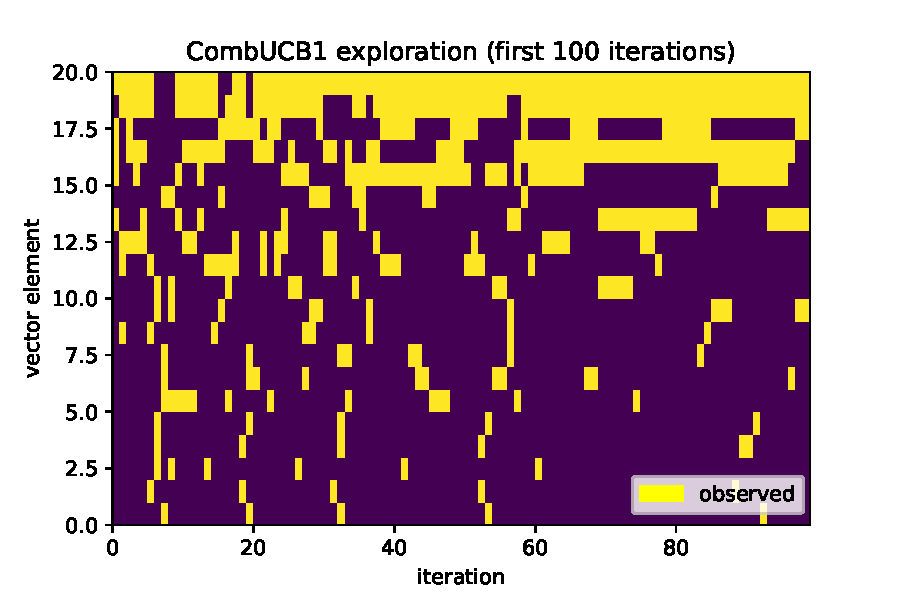
\includegraphics[width=10cm]{../plots/basicCombUCB1_100iters.pdf}
  \caption{CombUCB1 initial exploration...}
  \label{}
  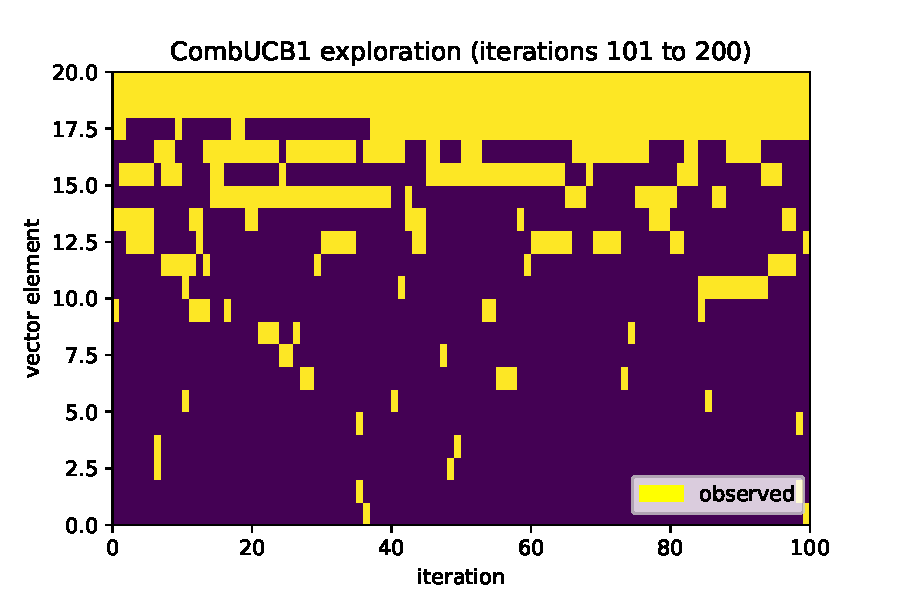
\includegraphics[width=10cm]{../plots/basicCombUCB1_100_200iters.pdf}
  \caption{...after the first 100 iterations...}
  \label{}
  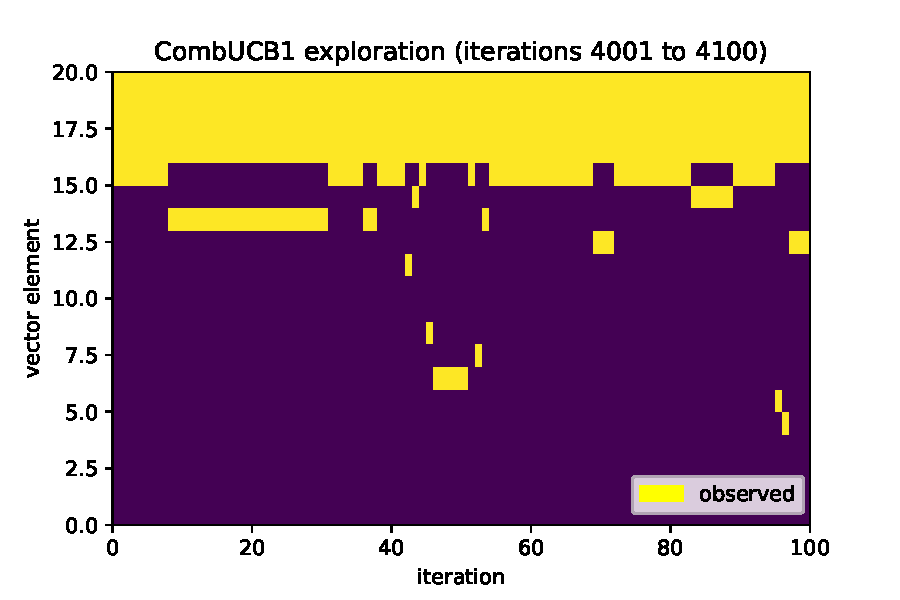
\includegraphics[width=10cm]{../plots/basicCombUCB1_4000_4100iters.pdf}
  \caption{...and after 4000 iterations}
  \label{}
\end{figure}

Figure 1 show how at the outset the algorithm is not confident what the expected value of any of the weights are and so it explores a lot. Figure 2 shows iterations 101 to 200, when the algorithm is starting to learn which elements have the highest expected value. Finally Figure 3 shows the algorithm after 4000 iterations at which time is has become quite confident which are the optimal paths, and does relatively little exploration.\\

The regret risk can be calculated as the sum of observed weights minus the sum of the weights of the top 5 elements of the vector. For 10,000 iterations this gives the following:\\

Optimal path reward = 42,399
Actual path reward = 41,905
Regret = 494\\

The algorithm performs very well at finding a near optimal solution.\\

\noindent \textbf{Adapted-FPL-TRiX}\\

Figures 4, 5 and 6 show the corresponding charts FPL-TRiX but adapted to find a maximum solution as opposed to a minimum solution. In fact this misses part of the essence of FPL-TRiX, which is that it adapts well in adversarial cases by keeping more of an open mind about trying the different options even once it has started to recognise the optimal solution. However, even though this is not exactly FPL-TRiX, it is interesting to include here as, with a bit of parameter tuning, it performs incredibly well in this situation. The reward and regret are:\\

Optimal path reward = 42,399
Actual path reward = 42,246
Regret = 153\\

Thus the algorithm outperforms CombUCB1. If you think of this slightly modified FPL-TRiX as part of the family of FPL-TRiX then it shows that this can be a nice adaptable framework to work in.\\

\begin{figure}%                 use [hb] only if necceccary!
  \centering
  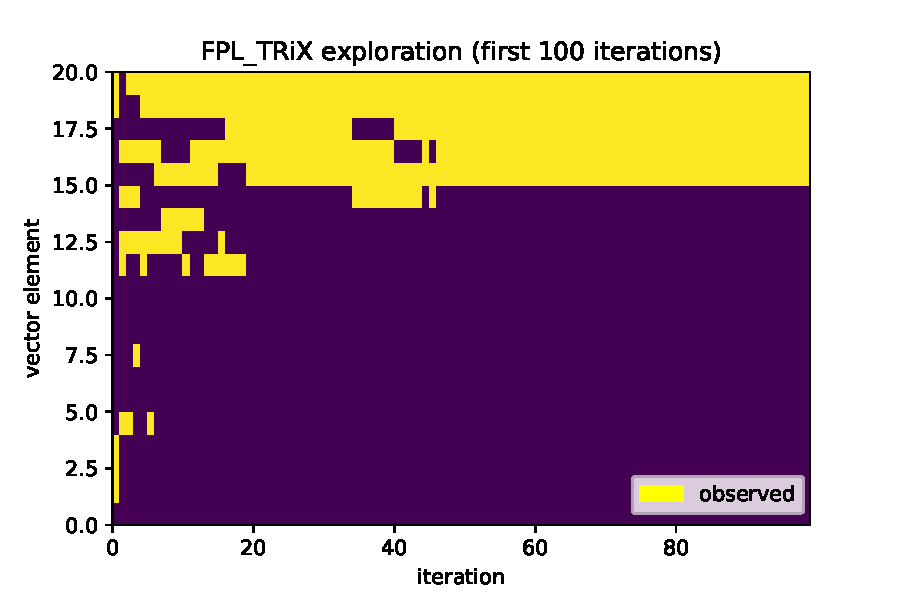
\includegraphics[width=10cm]{../plots/basicFPL_100iters.pdf}
  \caption{Adapted FPL-TRiX initial exploration...}
  \label{}
  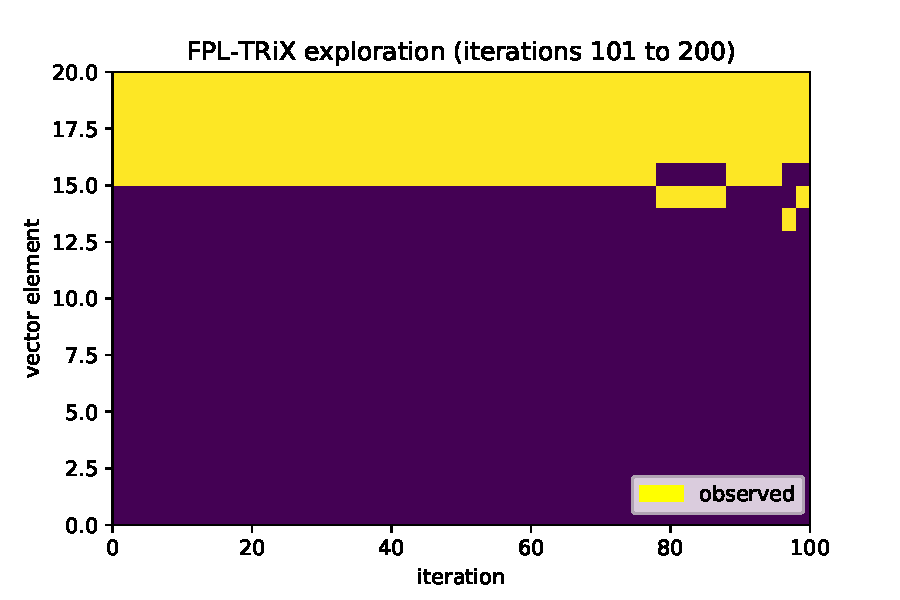
\includegraphics[width=10cm]{../plots/basicFPL_100_200iters.pdf}
  \caption{...after the first 100 iterations...}
  \label{}
  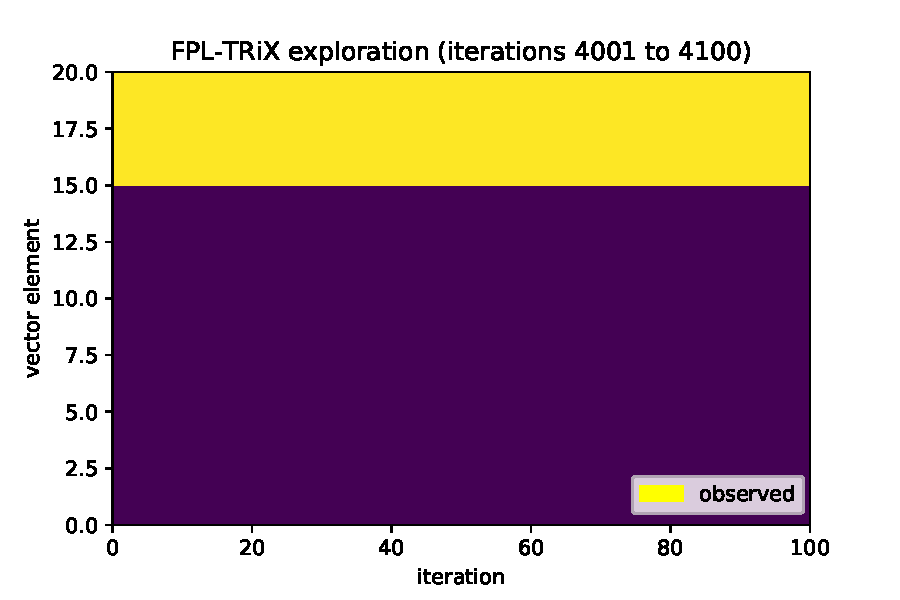
\includegraphics[width=10cm]{../plots/basicFPL_4000_4100iters.pdf}
  \caption{...and after 4000 iterations}
  \label{}
\end{figure}



DO WE WANT TO ALSO SHOW WHAT THE MATHEMATICAL BOUNDS ARE HERE???

Graphs showing how regret changes as inputs change (K, L, T etc)

Include adversarial case here?


\pagebreak

%----------------------------------------------------------------------------------------
%	NETWORK MINIMUM COST PATH PROBLEMS
%----------------------------------------------------------------------------------------

\section{Network minimum cost path problems}

A more sophisticated combinatorial problem to solve is a minimum cost path problem in a network. In this framework there are V vertices with edges in both directions between each pair of vertices, giving V $\times$ (V-1) edges in total. A path is chosen to travel from some starting vertex to an end vertex. The cost of each edge in the path is then stochastically drawn and the sum of these provides the total cost of the chosen path. The goal is to find the path with minimum expected cost. Clear application of this type of system in real-life could be any type of mass scale distibution such as electricity of communication networks.\\

Given the much more difficult combinatorial problem, this pushes the algorithms much harder. They will need to work out which higher cost edges are beneficial to use in order to take advantage of low cost paths than lead into or out of them. Thus the relative level of regret should be much higher than the previous more basic problem.\\

\subsection{Stochastic networks}

Firstly we look at how the algorithms perform in the stochastic setting, where the weights of the edges are drawn from truncated normal distributions limited to being between 0 and 1. Each edge has a different central point (i.e. different mean), and the variance was kept low at 0.1 so that there is a meaningful difference between the different paths.\\

With 10 vertices and observing 10,000 iterations the following costs were observed. This was after tuning the FPL-TRiX parameters, in particular reducing the gamma parameter to 0.01.\\

Optimal path cost = 2,269
UCB path cost = 3,742
FPL-TRiX path cost = 2,735\\

Perhaps surprisingly, FPL-TRiX is able to significantly outperform CombUCB1 in this situation. Figures 7, 8 and 9 show the edges of the optimal path at each iteration, and the edges of the paths chosen by CombUCB1 and FPL-TRiX. FPL-TRiX explores more at first allowing it to find the optimal path more quickly. Whereas CombUCB1 is led towards shorter paths at first, because if all edges start with similar wide confidence intervals then the paths with the least edges will appear to have the lowest costs. It is only after some time (around 200 iterations in this case) that CombUCB1 finds accurate enough estimates of the edges to work out that a longer path is in fact the optimal.\\

\begin{figure}%                 use [hb] only if necceccary!
  \centering
  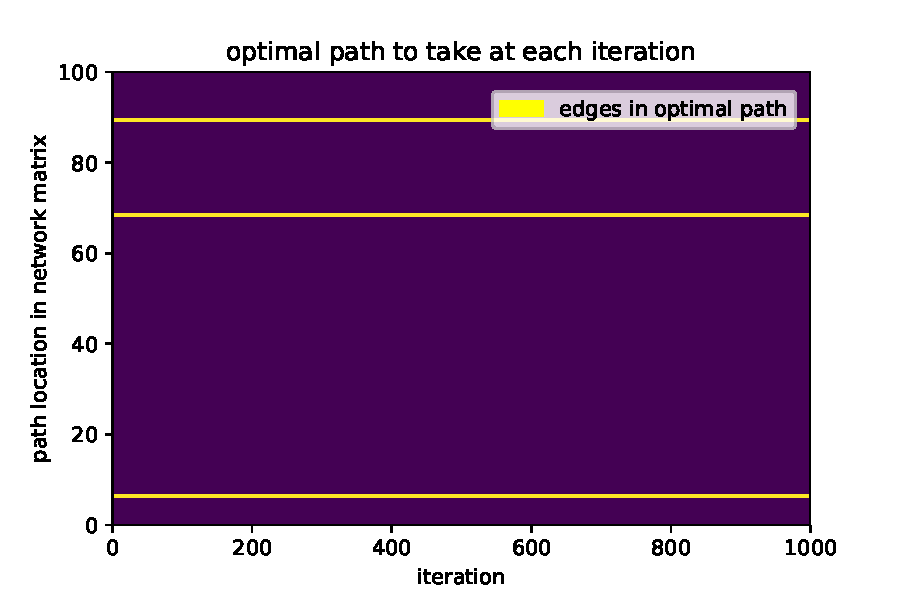
\includegraphics[width=8cm]{../plots/stoch_network_opt_paths.pdf}
  \caption{Optimal path of stochastic network}
  \label{}
  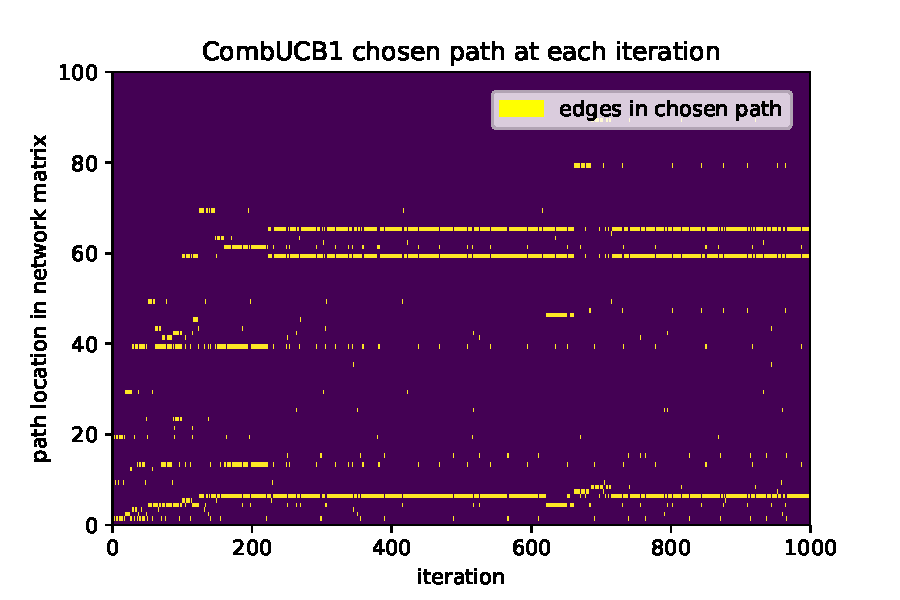
\includegraphics[width=8cm]{../plots/stoch_network_UCB1.pdf}
  \caption{CombUCB1 chosen paths}
  \label{}
  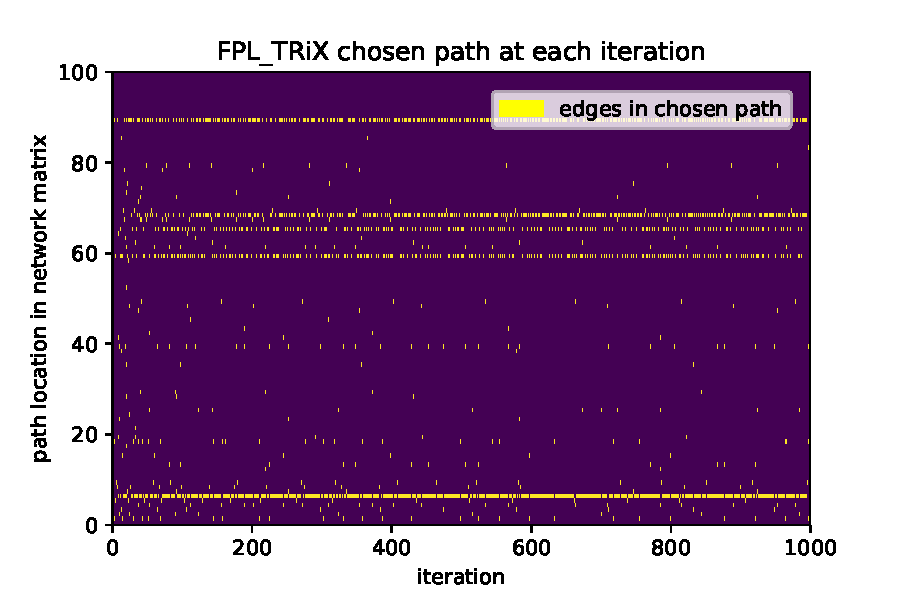
\includegraphics[width=8cm]{../plots/stoch_network_FPL.pdf}
  \caption{FPL-TRiX chosen paths}
  \label{}
\end{figure}

COULD TRY TO SET UP A MORE EXTREME SITUATION WHERE A LONGER PATH IS BEST AND COMBUCB1 TAKES AGES TO FIND IT




\subsection{Adversarial networks}

In this section we will progress to analysing the performance of the algorithms in an adversarial setting. 

Discussion on where FPL-TRiX can be advantageous (is FPL-TRiX best when in situations when 1. a longer path is best and 2. alternative routes are not much more costly so that it's extra exploration isn't too expensive??)

sCharts showing how the exploration changes between the two algorithms


\pagebreak

%----------------------------------------------------------------------------------------
%	PARAMETERS
%----------------------------------------------------------------------------------------

\section{Parameters}

Change FPL-TRiX Bt parameter to change exploration at different times.

Do this with knowledge of when system changes

Setup Bt to dynamically detect when the system changes and increase accordingly


Conclusion could be that parameter flexibility of FPL-TRiX allows it to increase or decrease searching as need be to perform better

\pagebreak

%----------------------------------------------------------------------------------------
%	THESIS CONTENT - APPENDICES
%----------------------------------------------------------------------------------------

\appendix % Cue to tell LaTeX that the following "chapters" are Appendices

% Include the appendices of the thesis as separate files from the Appendices folder
% Uncomment the lines as you write the Appendices


%\include{Appendices/AppendixB}
%\include{Appendices/AppendixC}

%----------------------------------------------------------------------------------------
%	BIBLIOGRAPHY
%----------------------------------------------------------------------------------------




\end{document}